\section{Vous êtes prêts ?}

13 nov. 2010

\begin{multicols}{2}

Bonjour,

C'est avec une certaine excitation que j'écris un nouveau message sur ce blog, mon sac est prêt, je repars pour un nouveau voyage le sac sur le dos, porté par les rencontres, la météo et les possibilités de transport locales.

La destination ? Une petite île à coté de l'Afrique.. Je vais à Madagascar pour trois semaines et demi.

Quant au programme, je suis encore incapable de vous le donner. Je vais attérir à Antananarivo vers le centre de l'île. Je pense ensuite descendre vers le Sud suivant les possibilités et remonter vers le nord pour la fin du voyage avant de redescendre vers la capitale. Comme d'habitude ce n'est qu'une prévision qui a toutes les chances d'être changée une fois là bas. Vous découvrirez donc la suite lorsque je la connaîtrai..

Ci-dessous une carte de l'île pour vous repérer dans les noms des villes que seront indiqués.

\hspace*{-0.65cm}
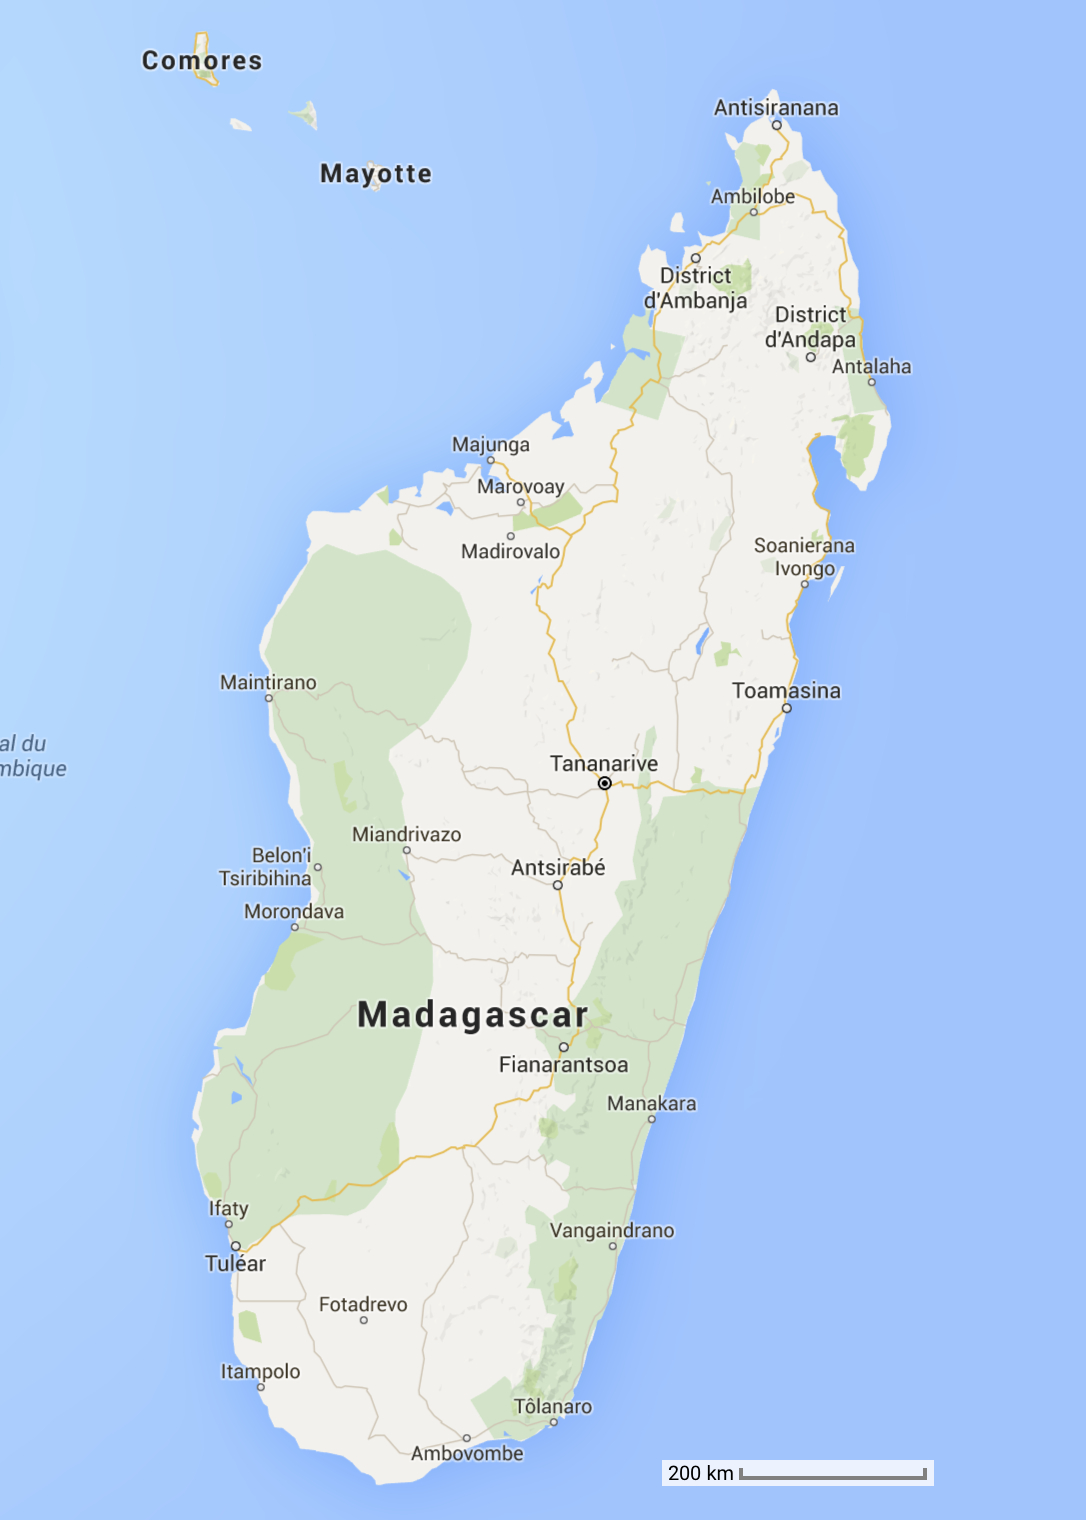
\includegraphics[width=4.8cm]{articles/Vous-etes-prets/madagascar.png}
Carte de Madagascar.

Je vous laisse, il me reste quelques petite choses à boucler avant de partir, alors à bientôt et n'hésitez pas à laisser des commentaires sous les billets, ça fait toujours chaud au coeur de les lire.

Au revoir.

\end{multicols}

\bigskip
\textbf{\textsc{Commentaires}}

\medskip
Didier a écrit le 13 nov. 2010 :
\begin{displayquote}
Bon voyage mec! Ca va être du bon...
PS: et sois un peu moins négligeant avec ton blog ;-)
A++
Didier
\end{displayquote}

\medskip
Nicoz et Emilie a écrit le 14 nov. 2010 :
\begin{displayquote}
Bon voyage !!
Profites en bien :)
Biz
Nico et Emilie
\end{displayquote}

\medskip
Macolu a écrit le 14 nov. 2010 :
\begin{displayquote}
Veinard ! Profites-en bien !
\end{displayquote}

\medskip
Dodo a écrit le 14 nov. 2010 :
\begin{displayquote}
Un petit voyage qui s'annonce bien ! Profite bien !
Et que la Dud attitude t'accompagne
La bise
\end{displayquote}

\medskip
Dovaline a écrit le 16 nov. 2010 :
\begin{displayquote}
Coucou Loulou,
Kiffes bien tes 4 semaines de vacances et fais nous rêver si peu par des commentaires et photos.
Gros Zoubis
\end{displayquote}

\medskip
Sonia a écrit le 18 nov. 2010 :
\begin{displayquote}
Coucou Étienne
Une p'tit bonjour de "Paris" où il pleut toujours.
Il y a combien de décalage horaire?
Profites et fais tourner :)
@+
Sonia
\end{displayquote}

\medskip
Etienne a écrit le 19 nov. 2010 :
\begin{displayquote}
Salut tout le monde, je suis aujourd'hui à Manakara et je pars pour Ambalavao ce soir. Le premier article sur ce blog risque d'attendre encore quelques jours mais il devrait être fort en récits et en photos car les paysages sont vraiment fabuleux. Pas de problèmes politiques en vue où je suis, n'écoutez pas les infos le problème semble en fait cantonné à une partie de la capitale et se règle surtout entre forces armées et normalement devrait se boucler autour d'une table dans les jour qui viennent. Je reste informé dans tous les cas pour éviter les endroits qui craignent.@ Sonia : L'heure de Mada est égale à l'heure de la France +2h, et comme on est vers le tropique le soleil se lève vers 5h30 et se couche vers 18h30.
\end{displayquote}


